\documentclass{article}

\usepackage[left=2cm,right=2cm,top=2cm,bottom=2cm]{geometry} 

\usepackage[utf8]{inputenc}   % otra alternativa para los caracteres acentuados y la "ñ"
\usepackage[           spanish % para poder usar el español
                      ,es-tabla % para los captions de las tablas
                       ]{babel}   
\decimalpoint %para usar el punto decimal en vez de coma para los números con decimales

%\usepackage{beton}
%\usepackage[T1]{fontenc}

\usepackage{parskip}
\usepackage{xcolor}

\usepackage{caption}

\usepackage{fancyvrb}

\usepackage{enumerate} % paquete para poder personalizar fácilmente la apariencia de las listas enumerativas

\usepackage{graphicx} % figuras
\usepackage{subfigure} % subfiguras

\usepackage{amsfonts}
\usepackage{amsmath}

\usepackage[formats]{listings}
\lstdefineformat{R}{~=\( \sim \)}
\lstset{basicstyle=\ttfamily,format=R}

\definecolor{gris}{RGB}{220,220,220}
	
\usepackage{float} % para controlar la situación de los entornos flotantes

\restylefloat{figure}
\restylefloat{table} 
\setlength{\parindent}{0mm}


\usepackage[bookmarks=true,
            bookmarksnumbered=false, % true means bookmarks in 
                                     % left window are numbered
            bookmarksopen=false,     % true means only level 1
                                     % are displayed.
            colorlinks=true,
            allcolors=blue,
            urlcolor=blue]{hyperref}
\definecolor{webblue}{rgb}{0, 0, 0.5}  % less intense blue


\title{\Huge SWAP: Servidor de disco NFS\vspace{10mm}}

\author{\huge David Cabezas Berrido \vspace{10mm} \\ 
  \huge dxabezas@correo.ugr.es \vspace{10mm}}

\begin{document}
\maketitle
\tableofcontents
\newpage

\section{Preparativos}

Creamos una nueva máquina virtual llamada \textbf{NFS-dxabezas}. Al igual que las otras máquinas, configuramos el doble adaptador de red
(NAT + Solo-Anfitrión), instalamos Ubuntu Server 18.04.1 y creamos un usuario \emph{dxabezas} con contraseña \emph{Swap1234}.
Comprobamos mediante PING que la máquina NFS tiene conexión con el resto de máquinas en la granja.

\section{Configurar servidor NFS}

Comenzamos creando la carpeta a compartir, y cambiamos el propietario y los permisos.

\begin{Verbatim}
sudo mkdir -p /datos/compartido
sudo chown nobody:nogroup /datos/compartido/
sudo chmod -R 777 /datos/compartido/
\end{Verbatim}

Comprobamos el propietario y los permisos que acabamos de asignar.

\begin{figure}[H]
	\centering
	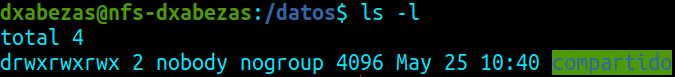
\includegraphics[width=110mm]{imgs/compartido-ls-l}
\end{figure}

Le damos permisos a M1 y M2 añadiendo la siguiente línea a \texttt{/etc/exports}.
\begin{Verbatim}
/datos/compartido/ 192.168.56.102(rw) 192.168.56.101(rw)
\end{Verbatim}

Finalmente, reiniciamos el servicio y comprobamos el estado.
\begin{figure}[H]
	\centering
	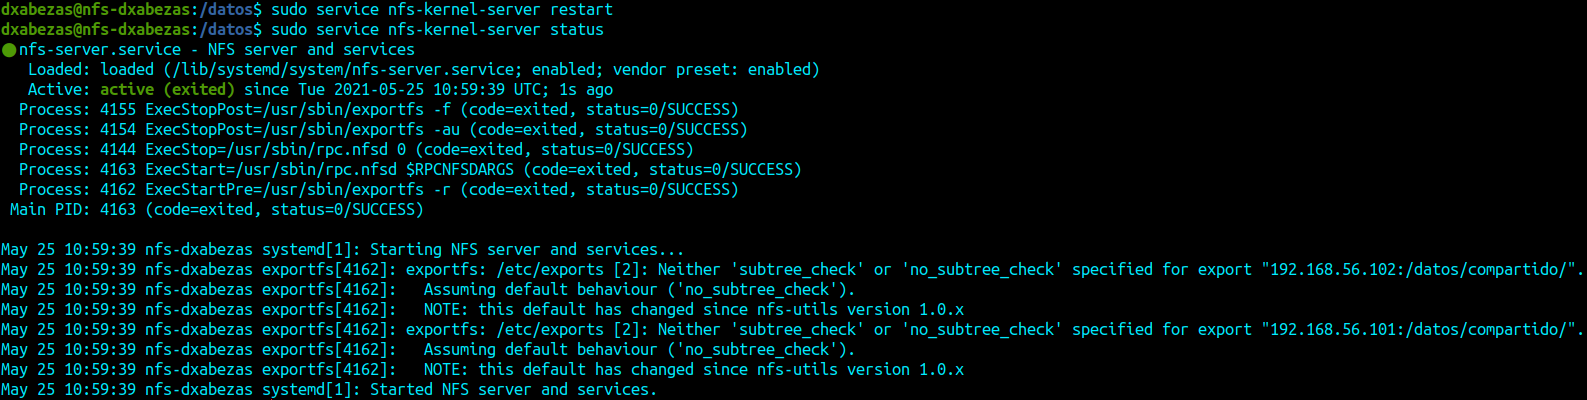
\includegraphics[width=180mm]{imgs/status}
	\caption{Todo parece estar correcto, teniendo en cuenta que estamos asumiendo la opción \texttt{no\_subtree\_check}. El subtree check consiste
	en comprobar que cada petición NFS solicita sólo archivos que están siendo exportados, para ello necesita información sobre el directorio
	padre.}
\end{figure}

\section{Configurar los clientes M1 y M2}

\section{Seguridad en el servidor NFS}

\end{document}
